\chapter{Teori}
\label{cha:theory}

\section{Punktmoln}
På senare år har det blivit möjligt att representera objekt i form av ett 3D-representerat punkt\-moln. Detta har blivit möjligt på grund av utvecklandet av kameror samt laserskannrar. Ett punktmoln är en mängd av punkter i ett tredimensionellt koordinatsystem som representerar ett objekt. Punkterna i punktmolnet representerar ofta de yttre kanterna av objektet \cite{point_cloud}.

Det finns två typer av punktmoln, ett så kallat komplett punktmoln och ett icke komplett punktmoln. Ett komplett punktmoln, se figur \ref{fig:point_cloud_torus}, betyder att punktmolnet innehåller samtliga punkter som behövs för att representera objektet. Ett icke komplett punktmoln, se figur \ref{fig:point_cloud_church}, betyder att punktmolnet endast representerar en sida av objektet och alltså inte innehåller tillräckligt med punkter för att representera hela objektet.

\begin{figure}[H]
	\centering
	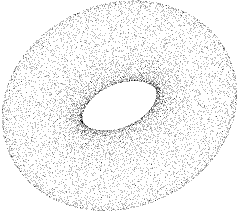
\includegraphics[width=30mm]{figures/Point_cloud_torus1.png}
	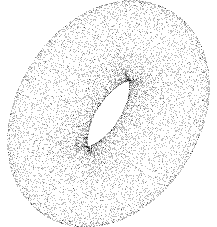
\includegraphics[width=30mm]{figures/Point_cloud_torus2.png}
	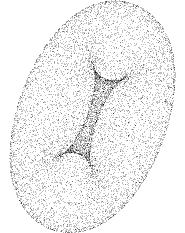
\includegraphics[width=30mm]{figures/Point_cloud_torus3.png}
	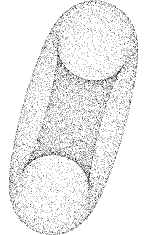
\includegraphics[width=30mm]{figures/Point_cloud_torus4.png}
	\caption{Ett komplett punktmoln som representerar ett torusobjekt.}
	\label{fig:point_cloud_torus}
\end{figure}

\begin{figure}[H]
	\centering
	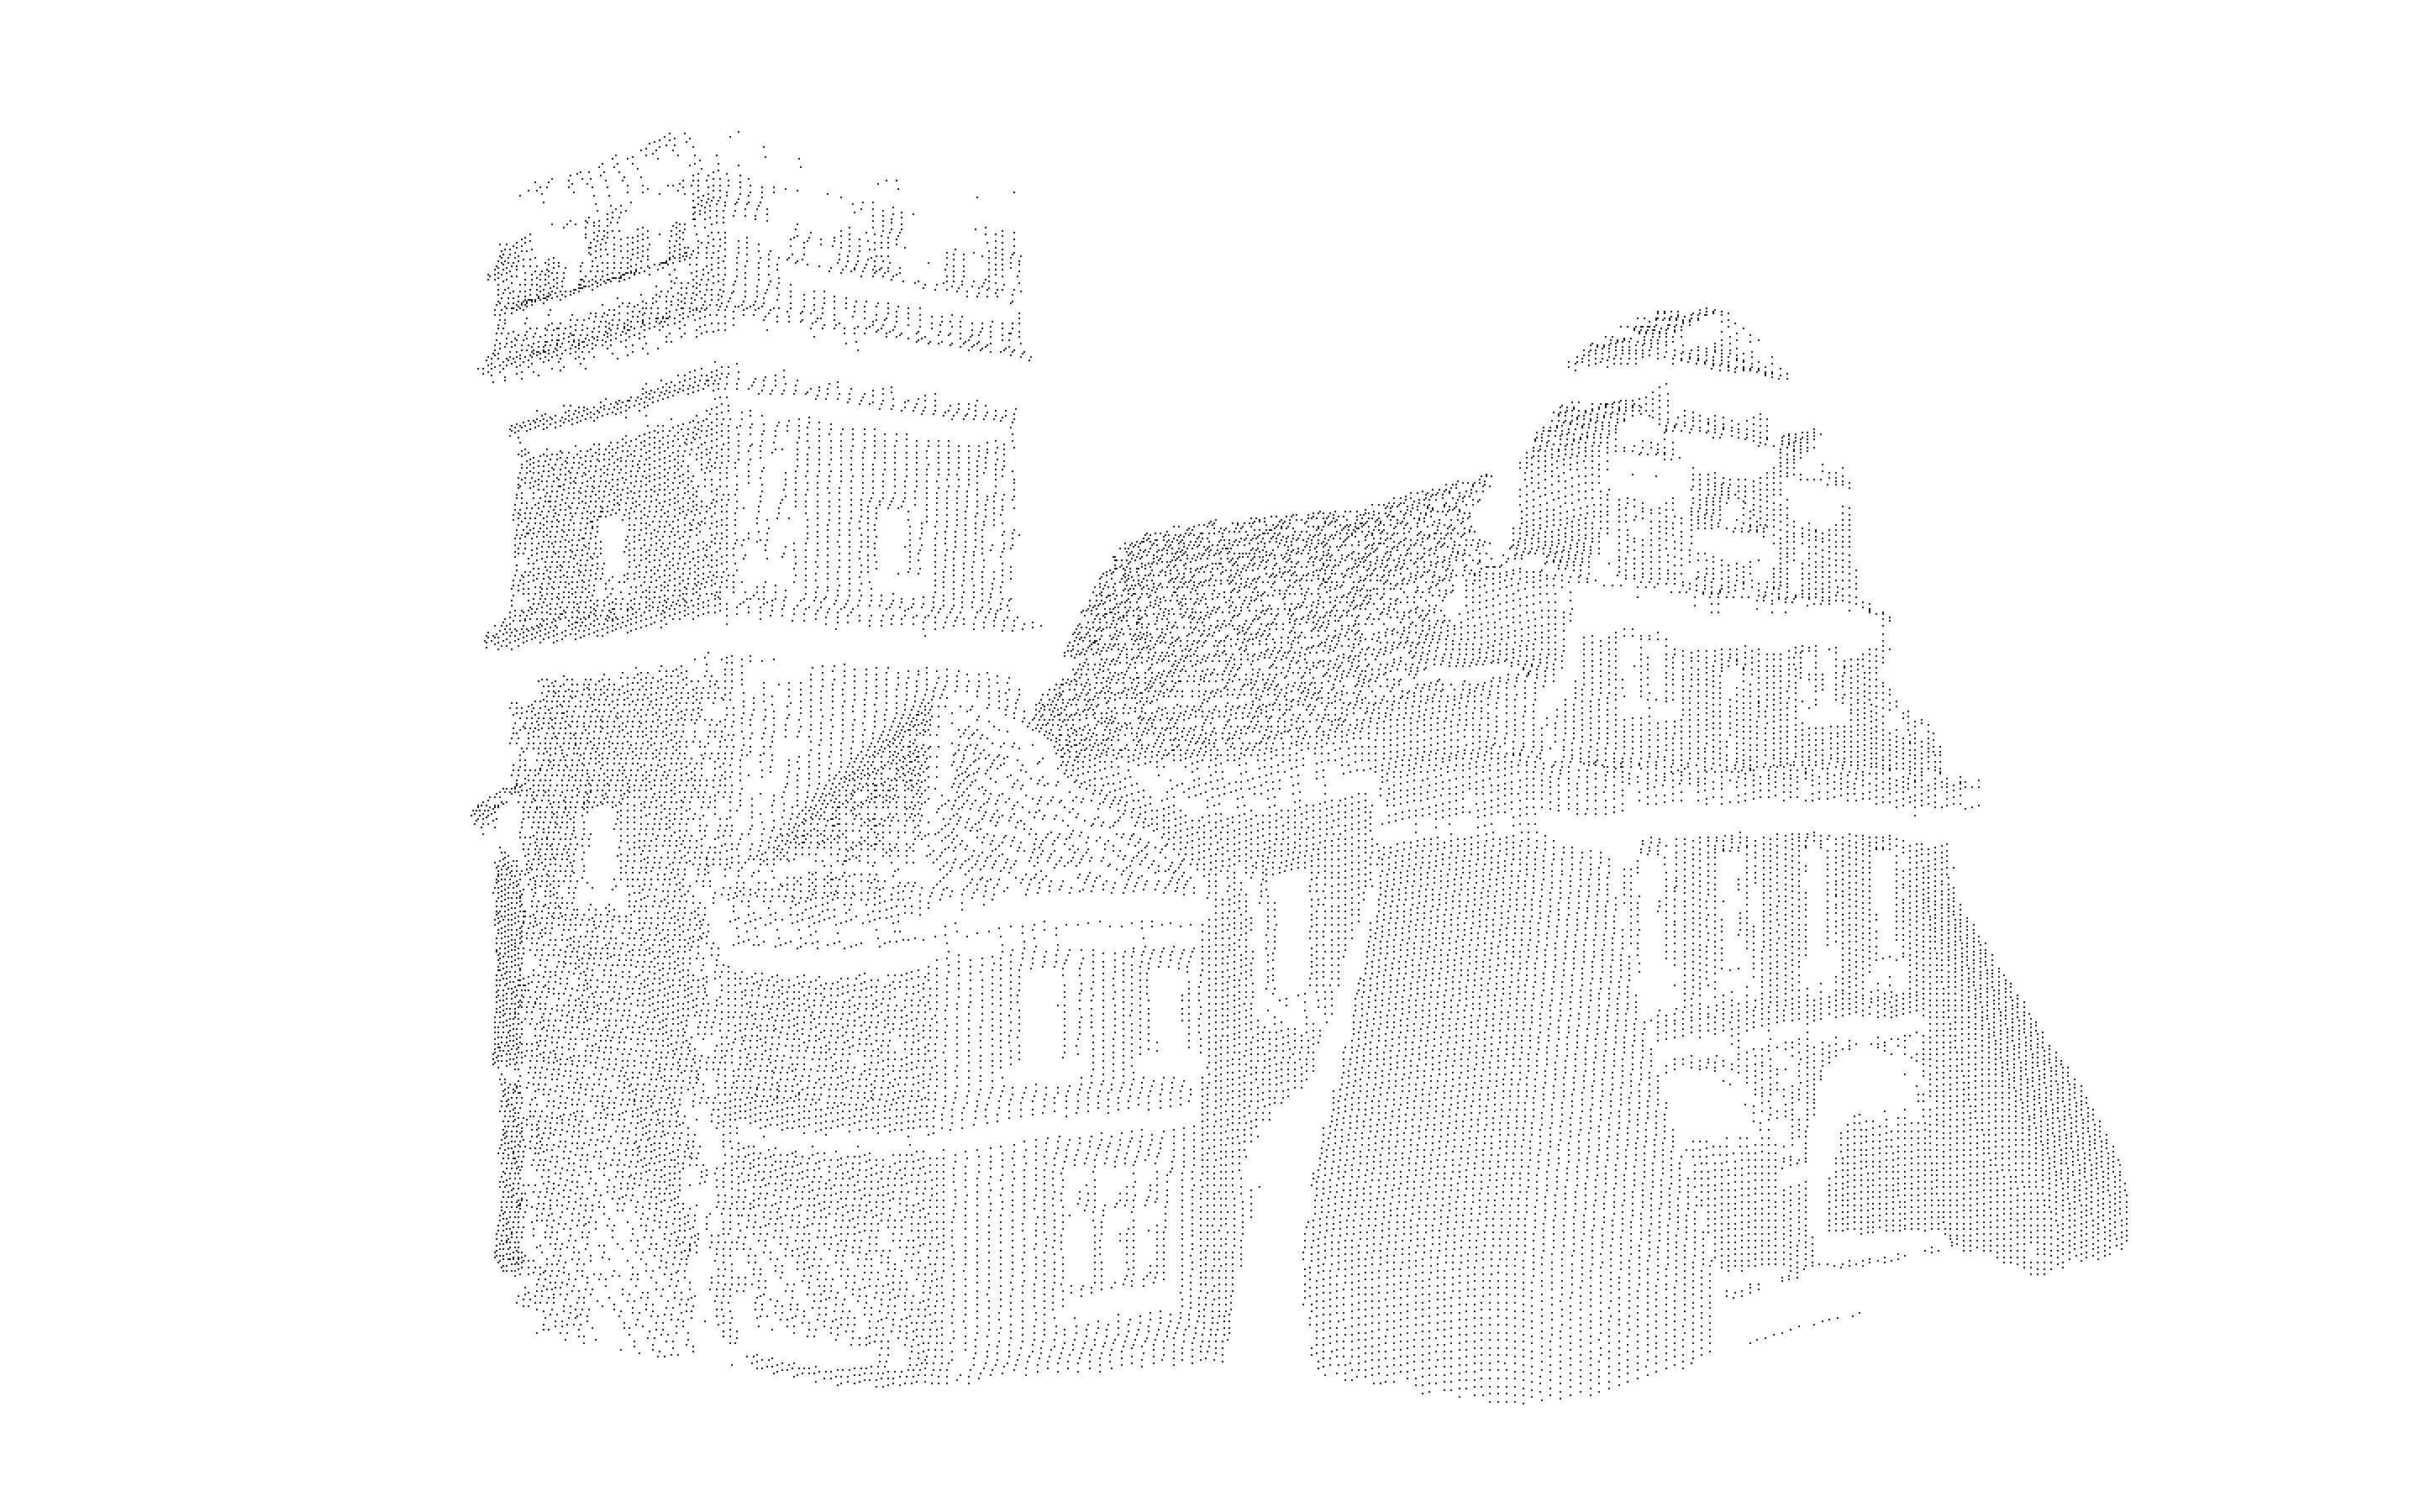
\includegraphics[width=100mm]{figures/icke_komplett_moln_kyrka.png}
	\caption{Ett icke komplett punktmoln som representerar en del av en kyrka.}
	\label{fig:point_cloud_church}
\end{figure}

\section{Point Cloud Library}

Point Cloud Library (PCL) är ett bibliotek till C++ som bidrar med algoritmer till att behandla 3D-objekt. PCL innehåller bland annat algoritmer för:

\begin{itemize}
	\item filtrering
	\item registrering
	\item segmentering
	\item modellanpassning
	\item ytrekonstruering
	\item funktionsestimering.
\end{itemize}
PCL är alltså ett bibliotek avsett att ge stöd till att behandla punktmolnsdata, i form av olika bearbetningsalgoritmer \cite{rusu20113d}.

PCL använder sig av ett eget visualiseringsbibliotek för att visualisera punktmoln. Visualiseringsbiblioteket i PCL integrerar med visualiseringsverktyget VTK \cite{VTK_book}\cite{rusu20113d}.

Nedan beskrivs de olika algoritmerna som PCL innehåller. De algoritmer som beskrivs är de algoritmer som är relevanta för detta projekt.

\subsection{Filtrering}
PCLs filtreringsbibliotek innehåller algoritmer för att filtrera bort skräppunkter från ett punktmoln. Dessa skräppunkter kan uppstå vid skanning av ett objekt eftersom avståndskameran kan reagera på bakgrunden och inte bara på objektet. Detta gör att skräppunkter infaller i punkmolnet. För att kunna behandla punktmolnet måste dessa skräppunkter först filtreras bort.

PCL har stöd för flera olika metoder för filtrering. Första steget i vår filtrering är att ta bort alla punkter som ligger utanför ett visst intervall av koordinater. Syftet med detta är att ta bort sådant som måste ligga utanför det skannade objektet. I nästa steg kontrolleras det för varje punkt hur många grannar den punkten har inom en viss radie. Alla punkter som har under ett visst antal grannar tas bort vilket leder till att enstaka punkter som inte ligger i närheten av något objekt tas bort \cite{pcl_filtering}.

För att undvika att punktmoln blir för stora, det vill säga får för många punkter så att de tar för lång tid att behandla, kan nedsampling (från eng. \textit{"down sampling"}) användas för att ta bort punkter och samtidigt uppskatta den yta som representeras så nära som möjligt. För att göra detta i PCL delas punktmolnet som ska nedsamplas in i voxels, vilket kan ses som att punktmolnet delas in i ett antal kuber. Sedan ersätts alla punkter i varje kub med en punkt som ligger i centrum för alla punkterna i kuben. På detta sätt ges en nära uppskattning av den representerade ytan med mycket färre punkter än det ursprungliga punktmolnet \cite{voxel_grid}.
 

\subsection{Registrering}
Att kombinera två punktmoln till ett punktmoln som innehåller samma information kallas för att "registrera punktmoln". Detta är en komplicerad process där både translationen och rotationen, runt alla axlar, kan behöva ändras. Målet med parvis registrering, registrering av två punktmoln, är att flytta ett moln så att alla punkter som överlappar i de två separata molnet, överlappar i resultatmolnet. I PCL finns ett registreringsbibliotek som innehåller algoritmer för registrering\cite{pcl_registration}. För mer information angående registreringen och dess algoritmer, se Michael Karlssons individuella utredning i kapitel \ref{cha:indiv-report-karlsson}. 

%Att anpassa olika punkter i ett punktmoln så att de representerar en komplett modell över objektet kallas för punktmolnsregistrering. Registrering är ett stort problem och PCL erbjuder ett registreringsbibliotek för ändamålet. Målet med registreringen är att hitta de relativa positionerna och orienteringarna för de separata punktmolnen (tagna från olika vyer) så att varje punkt i respektive moln överlappar perfekt med varandra \cite{pcl_registration}. För mer information angående registreringen och dess algoritmer, se Michaels Karlssons individuella utredning i kapitel \ref{cha:indiv-report-karlsson}.

För att registrera punktmoln finns ett antal olika algoritmer med olika för- och nackdelar. En vanlig algoritm är \textit{Iterative Closest Point} (ICP). Det är en så kallad parvis registreringsalgoritm som registrerar enbart ett punktmoln till ett annat. ICP går ut på att minimera summan av avståndet från varje punkt i det ena punktmolnet till varje punkt i det andra punktmolnet.

För att begränsa antalet punkter som måste beräknas används parametern \textit{Max correspondence distance} så att enbart de punkter inom avståndet räknas in i summan för varje punkt. \textit{Transformation epsilon} är ett mått på hur mycket transformationen för punktmolnet som ska matchas in får ändras för varje iteration. Genom att öka detta epsilon kan, vid behov, algoritmen flytta punktmolnet längre och därmed nå sitt mål på färre iterationer. Nackdelen med ett för högt epsilon är dock att punktmolnet kan flyttas förbi optimum som därmed slösar tid. Slutligen kan \textit{Max iterations} användas för att avgöra hur många gånger algoritmen ska köras för varje parvis registrering. Genom att öka antalet iterationer ökar tidsåtgången men resultatet förbättras också \cite{pcl_icp_docs}.

\subsection{Ytrekonstruering}
För att återskapa ytor från en 3D-modell används PCLs ytrekonstrueringsbibliotek. I projektets sammanhang betyder det att ett punktmoln rekonstrueras till en vattentät modell. De algoritmer som biblioteket tillhandahåller används i projektet för att generera en mesh utifrån ett komplett punktmoln \cite{pcl_surface_reconstruction}.  

%%PCLs ytrekonstrueringsbibliotek innehåller algoritmer för att rekonstruera de ursprungliga ytorna från 3D-skanningar. Beroende på uppgiften kan PCL till exempel rekonstruera en ojämn yta till en jämn, en meshrepresentation av ett komplett punktmoln eller en yta med normaler \cite{pcl_surface_reconstruction}.

%Att rekonstruera en ojämn yta till en jämn kan vara viktigt om molnet är brusigt, eller om det består av flera skanningar som inte är perfekt anpassade. PCLs ytrekonstrueringsbibliotek kan även skapa en konkav modell av ett punktmoln. Detta kan vara bra om till exempel gränserna i ett punktmoln behöver extraheras \cite{pcl_surface_reconstruction}.

Meshning av ett punktmoln görs efter att punktmolnen registrerats så de bildar ett komplett punktmoln. Att skapa en meshrepresentation av ett komplett punktmoln innebär att skapa en yta utan punkter. Meshrepresentationen av punktmolnet är alltså en vattentät 3D-modell uppbyggd av polygoner. Den algoritm som används för att mesha ett punktmoln i projektet är en trianguleringsalgoritm (Poisson surface reconstruction) som körs på ett punktmoln med normaler för att erhålla en yta baserad på grannarna till respektive punkt. För detta krävs alltså ett punktmolnsobjekt som innehåller normalerna till varje punkt i punktmolnet. I detta punktmoln med normaler kan sedan önskade parametrar sättas innan själva trianguleringsalgoritmen körs för att generera den önskade meshen \cite{pcl_surface_reconstruction}\cite{pcl_triangulation_algorithm}. 


\section{3D-skrivare}
En 3D-skrivare kan användas för att skriva ut 3D-objekt i plast utifrån modeller i en dator. För att kunna göra detta har skrivaren ett styrkort som exekverar så kallad G-code \cite{gcode}. Denna G-code beskriver vilka motorer som ska flyttas och hur mycket. En 3D-modell som är sparad i datorn, i form av en mesh, måste alltså behandlas genom att använda en algoritm för att generera G-code utifrån modellen. Detta görs ofta genom en typ av programvara som kallas för slicer. Namnet kommer av att programmet delar upp modellen i olika lager och sedan genererar hur skrivaren måste röra sig för att skriva ut ett lager. På detta sätt byggs sedan hela den ursprungliga modellen upp lager för lager. Två vanliga slicer-programvaror är \textit{Cura} \cite{cura} och \textit{Slic3r} \cite{slic3r}.

\section{Systemanatomi}
En systemanatomi är en beskrivning av ett systems funktionalitet. Ofta består en systemanatomi av en graf, där noder representerar systemets olika funktioner och bågar representerar beroenden. Systemanatomin säger ingenting om hur systemet ska implementeras utan ger en utvecklingsgrupp en bra översikt av vad systemet ska göra. En systemanatomi kan inte ersätta andra modeller men är ett bra komplement.  


%%En systemanatomi är en visuell beskrivning av ett system som används för att bättre förstå systemet och dess interna beroenden. En systemanatomi säger inget om hur systemet ska implementeras eller hur det är uppbyggt rent tekniskt utan det enda den säger är vilken funktionalitet systemet ska innehålla och vad systemet ska kunna utföra. Därför kan en systemanatomi inte ersätta andra modeller eller designverktyg utan det är enbart ett annat sätt att beskriva systemet och vad det ska göra \cite{system_anatomy}.


\section{Hållbar utveckling}

Hållbar utveckling är en relevant aspekt i dagens utveckling av programvaror eftersom de används kontinuerligt av samhället. En programvara som utvecklats kan både hjälpa samhället framåt men också påverka samhället negativt beroende på hur den producerats och hur den används \cite{raturi2014developing}.

Hållbarhet definieras som "förmåga att uthärda" och "bevara funktionen hos ett system under en utsträckt tidsperiod". Att analysera hållbarhet hos ett mjukvarusystem innebär för de som utvecklar systemet att ha dessa fyra områden i åtanke \cite{lago2015framing}:

\begin{itemize}
	\item Ekonomiskt -  Systemet ska bevara kapital och värde.
	\item Socialt - Systemet ska underhålla samhället.
	\item Miljö - Systemet ska skydda den mänskliga välfärden genom att skydda naturens tillgångar.
	\item Tekniskt - Systemet ska utvecklas för att stödja långtidsanvändning.
\end{itemize}
En mer ingående beskrivning om hur vårt projekt främjar hållbar utveckling diskuteras i avsnitt \ref{disc:hållbar_utveckling}.


%%%%%%%%%%%%%%%%%%%%%%%%%%%%%%%%%%%%%%%%%%%%%%%%%%%%%%%%%%%%%%%%%%%%%%
%%% theory.tex ends here
